\documentclass[11pt,a4paper]{article}
\usepackage[utf8]{inputenc}
\usepackage[spanish]{babel}
\usepackage{amsmath}
\usepackage{amsfonts}
\usepackage{amssymb}

\usepackage[hyphens]{url}
\usepackage{hyperref}

\usepackage{float}
\usepackage{graphicx}
\usepackage{geometry}
\usepackage{hyperref}
\usepackage{apacite}

\newgeometry{left=3cm, right=3cm, top=2.5cm, bottom=2.5cm}



\usepackage{listings}
\usepackage{xcolor}

\definecolor{codegreen}{rgb}{0,0.6,0}
\definecolor{codegray}{rgb}{0.5,0.5,0.5}
\definecolor{codepurple}{rgb}{0.58,0,0.82}
\definecolor{backcolour}{rgb}{0.95,0.95,0.92}

\lstdefinestyle{mystyle}{
	backgroundcolor=\color{backcolour},   
	commentstyle=\color{codegreen},
	keywordstyle=\color{magenta},
	numberstyle=\tiny\color{codegray},
	stringstyle=\color{codepurple},
	basicstyle=\ttfamily\footnotesize,
	breakatwhitespace=false,         
	breaklines=true,                 
	captionpos=b,                    
	keepspaces=true,                 
	numbers=left,                    
	numbersep=5pt,                  
	showspaces=false,                
	showstringspaces=false,
	showtabs=false,                  
	tabsize=2
}

\lstset{style=mystyle}



\begin{document}
\begin{titlepage}
\centering


{\bfseries\LARGE UNIVERSIDAD NACIONAL DEL ALTIPLANO\par}
{\scshape\LARGE Facultad de Ingeniería Mecánica Eléctrica, Electrónica y Sistemas\par}
{\scshape\LARGE Escuela Profesional de Ingeniería de Sistemas\par}
\vspace{1cm}
{
\includegraphics[width=0.6\textwidth]{images/1-unap.png}\par}
\vspace{0.5cm}
{\bfseries\LARGE Práctica N°3\par}
\vspace{1cm}
{\LARGE Docente: Mg. Aldo Hernan Zanabria Galvez \par}

{\LARGE Alumno: Yoel Nhelio Canaza Chagua \par}
\vspace{1cm}
{\LARGE Curso: \par}
{\LARGE Programación Orientada a Objetos II \par}
\vspace{1cm}
{\LARGE CICLO III – SEMESTRE 2023 – II \par}
{\LARGE PUNO, PERÚ \par}
{\LARGE 2023 \par}


\end{titlepage}

\section{Del siguiente código:}

\begin{lstlisting}[language=Python, style=mystyle, caption={Código base sin modificaciones.}]


class Estudiante:
    def __init__(self, nombre, edad, curso):
        self.nombre = nombre
        self.edad = edad
        self.curso = curso

    def mostrar_informacion(self):
        print(f"Nombre: {self.nombre}")
        print(f"Edad: {self.edad} años")
        print(f"Curso: {self.curso}")

# Crear instancias de la clase Estudiante
estudiante1 = Estudiante("Juan", 20, "Ingeniería")
estudiante2 = Estudiante("Ana", 22, "Ciencias de la Computación")

# Mostrar la información de los estudiantes
print("Información del Estudiante 1:")
estudiante1.mostrar_informacion()

print("\nInformación del Estudiante 2:")
estudiante2.mostrar_informacion()


\end{lstlisting}

\subsection{Crea una nueva instancia de la clase Estudiante con tus propios datos y muestra su información utilizando el método mostrar\_informacion.}

\begin{figure}[H]
    \centering
    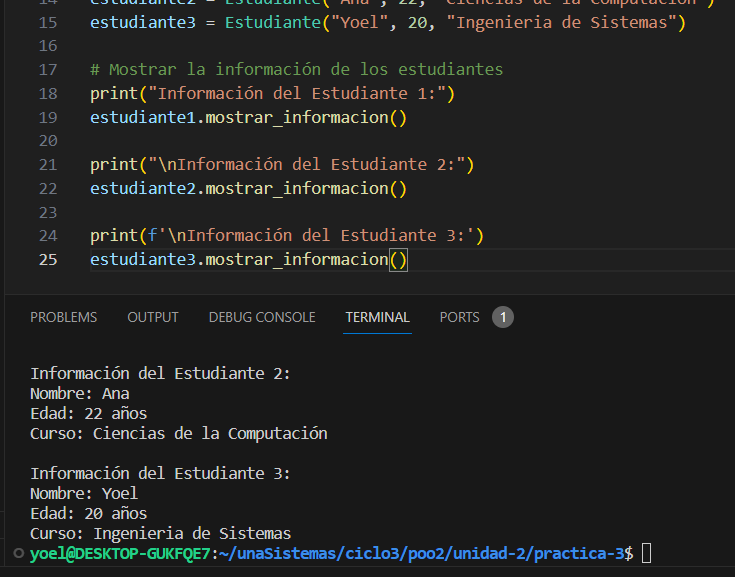
\includegraphics[width=0.9\linewidth]{images/2.png}
    \caption{Creando nueva instancia y mostrando la información de esa instancia}
    \label{fig:enter-label}
\end{figure}

\subsection{Añade un nuevo método a la clase Estudiante llamado cumpleaños que incrementa la edad del estudiante en 1 año. Luego, utiliza este método con una de las instancias creadas para simular el paso de un año.}

\begin{figure}[H]
    \centering
    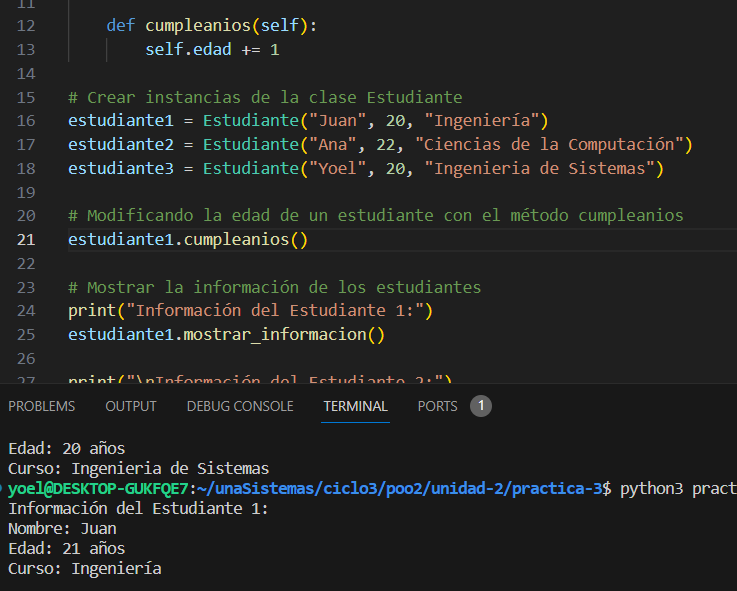
\includegraphics[width=0.6\linewidth]{images/3.png}
    \caption{Modificando la edad de estudiante1 con el método 'cumpleanios'}
    \label{fig:enter-label}
\end{figure}

\subsection{Crea una clase adicional llamada Curso que tenga un atributo para el nombre del curso y un método para mostrar la información del curso. Luego, modifica la clase Estudiante para que tenga un atributo de tipo Curso y muestra la información del estudiante y el curso al que pertenece.}

\begin{figure}[H]
    \centering
    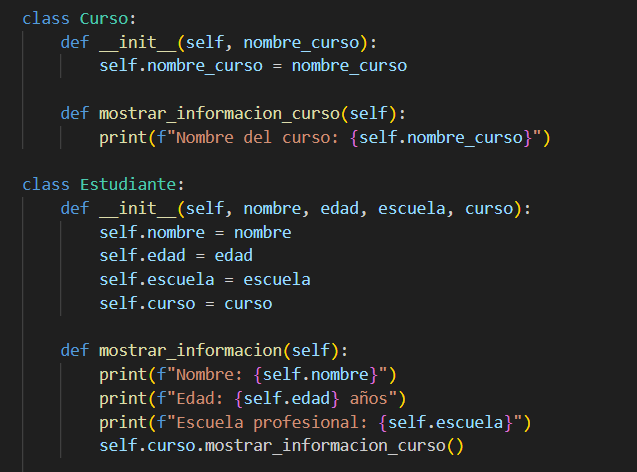
\includegraphics[width=0.6\linewidth]{images/4.png}
    \caption{Creando la clase Curso y modificando la clase Estudiante para que tenga un atributo de tipo Curso y su función 'mostrar\_informacion' también permita mostrar el nombre del curso}
    \label{fig:enter-label}
\end{figure}

\begin{figure}[H]
    \centering
    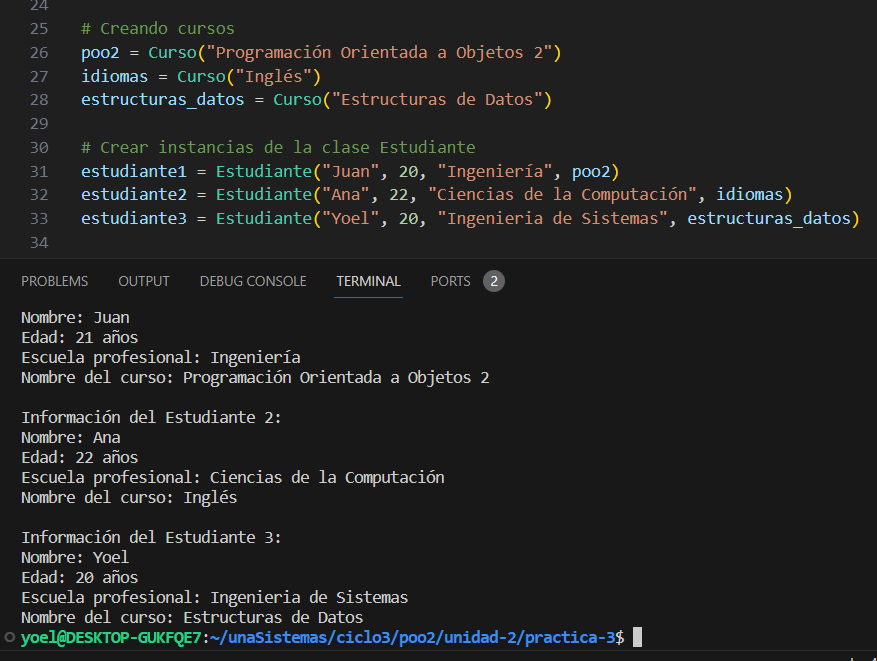
\includegraphics[width=1\linewidth]{images/5.png}
    \caption{Creando los cursos para luego pasarlos como argumentos en la inicialización de las instancias de la clase Estudiante}
    \label{fig:enter-label}
\end{figure}

\subsection{Implementa una clase llamada Universidad que tenga una lista de estudiantes. Agrega métodos para añadir un estudiante nuevo, mostrar la cantidad total de estudiantes y mostrar la información de todos los estudiantes.}

\begin{figure}[H]
    \centering
    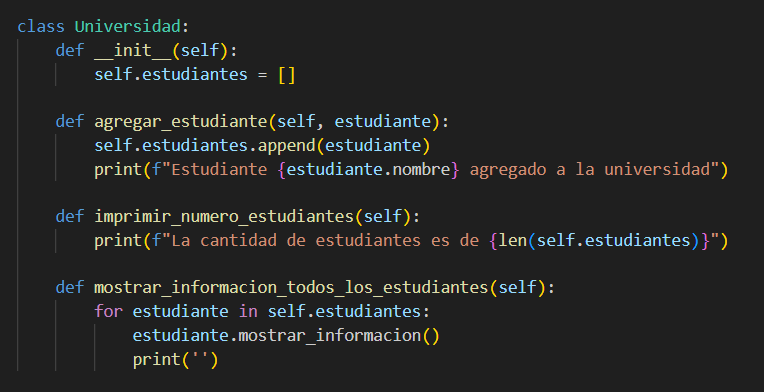
\includegraphics[width=0.8\linewidth]{images/6.png}
    \caption{Implementando una clase llamada Universidad con una lista de estudiantes, y con métodos para añadir estudiantes nuevos, mostrar la cantidad de estudiantes, y mostrar la información de todos los estudiantes}
    \label{fig:enter-label}
\end{figure}

\begin{figure}[H]
    \centering
    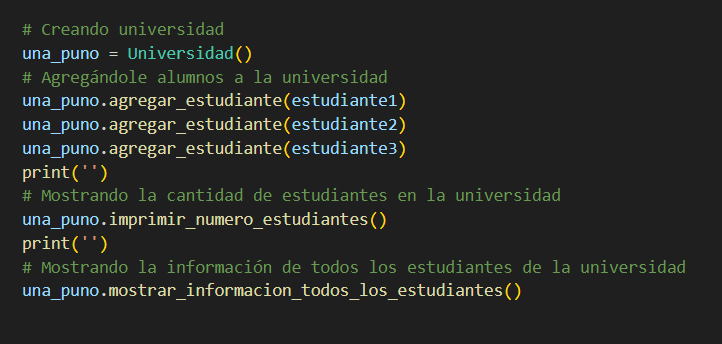
\includegraphics[width=1\linewidth]{images/7.png}
    \caption{Creando una instancia de la clase Universidad, agregándole alumnos y mostrando la información de todos sus estudiantes}
    \label{fig:enter-label}
\end{figure}

\begin{figure}[H]
    \centering
    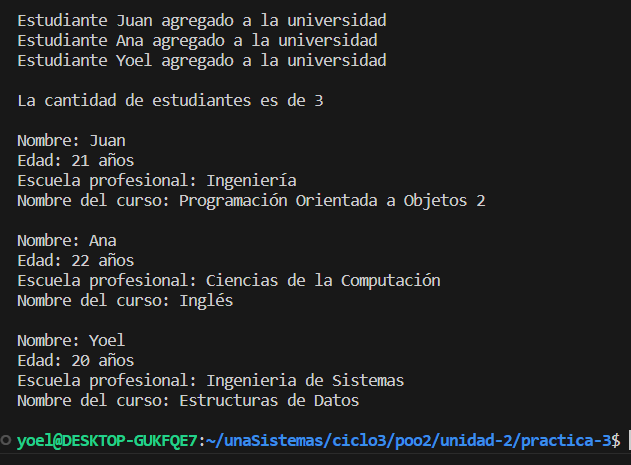
\includegraphics[width=1\linewidth]{images/8.png}
    \caption{}
    \label{fig:enter-label}
\end{figure}

\subsection{Define un método en la clase Estudiante llamado es\_mayor\_de\_edad que devuelve True si el estudiante tiene 18 años o más, y False en caso contrario. Luego, utiliza este método para determinar si un estudiante es mayor de edad.}

\begin{figure}[H]
    \centering
    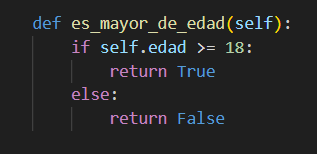
\includegraphics[width=0.5\linewidth]{images/9.png}
    \caption{Definiendo el método solicitado}
    \label{fig:enter-label}
\end{figure}

\begin{figure}[H]
    \centering
    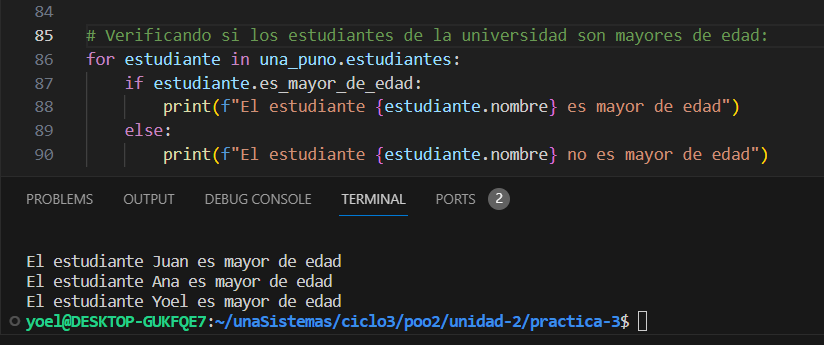
\includegraphics[width=1\linewidth]{images/10.png}
    \caption{Utilizando ese método para saber si los estudiantes de la intancia una\_puno de la clase Universidad son mayores de edad}
    \label{fig:enter-label}
\end{figure}

\section{Preguntas}
\subsection{¿Cuál es la ventaja de utilizar la programación orientada a objetos en comparación con otros enfoques?}

La programación orientada a objetos permite, mediante la abstracción, modelar problemas de manera más cercana a cómo se perciben en el mundo real, facilitando la comprensión del código y su mantenimiento.

También facilita la reutilización de código mediante el concepto de clases y objetos, la creación de módulos independientes y bien definidos (cada clase representa un módulo que encapsula su propia lógica y datos), 

Además, el encapsulamiento mejora la seguridad y facilita el mantenimiento del código, ya que los cambios internos no afectan al resto del código. La herencia fomenta la reutilización del código. Y el polimorfismo nos permite tratar objetos de clases diferentes de manera uniforme.

\subsection{¿Cuál es la diferencia entre una clase y una instancia en programación orientada a objetos?}

 Una clase es como un plano o una plantilla que define cómo deben ser los objetos, mientras que una instancia es un objeto específico creado a partir de esa plantilla, con sus propias características y comportamiento. Es decir, la clase proporciona la estructura y el diseño, y las instancias son ejemplos concretos basados en esa estructura.

\subsection{¿Por qué es importante encapsular datos en la programación orientada a objetos?}

La encapsulación nos ayuda a proteger los datos al limitar el acceso directo a ellos. Solo los métodos definidos en la propia clase pueden manipular los datos internos, evitando modificaciones no deseadas o errores accidentales. Al encapsular datos, se pueden aplicar restricciones y validaciones dentro de los métodos de la clase. Esto asegura que los datos se mantengan en un estado coherente y válido, evitando situaciones inconsistentes.

\subsection{Explica el concepto de herencia y proporciona un ejemplo en el contexto de la programación orientada a objetos.}

La herencia permite que una clase (llamada clase derivada o subclase) herede atributos y métodos de otra clase (llamada clase base o superclase). La herencia facilita la reutilización de código y la creación de jerarquías de clases, donde las subclases pueden extender o especializar el comportamiento de las superclases.

\begin{lstlisting}[language=Python, style=mystyle, caption={Ejemplo de herencia en Python.}]


class Vehiculo:
    def __init__(self, marca, modelo):
        self.marca = marca
        self.modelo = modelo

    def obtener_informacion(self):
        return f"{self.marca} {self.modelo}"

class Automovil(Vehiculo):
    def __init__(self, marca, modelo, puertas):
        # Llamamos al constructor de la clase base para inicializar marca y modelo
        super().__init__(marca, modelo)
        # Atributo específico de la subclase
        self.puertas = puertas

    def obtener_informacion(self):
        # Sobreescribimos el método de la clase base para agregar información específica
        return f"{self.marca} {self.modelo}, {self.puertas} puertas"

auto = Automovil("Toyota", "Corolla", 4)
print(auto.obtener_informacion())

\end{lstlisting}

\begin{figure}[H]
    \centering
    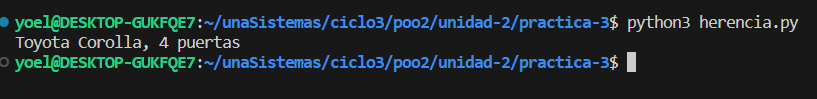
\includegraphics[width=0.6\linewidth]{images/11.png}
    \caption{La salida del código anterior}
    \label{fig:enter-label}
\end{figure}


\subsection{¿Cuándo deberías usar la programación orientada a objetos en lugar de otros paradigmas de programación?}

Cuando necesitemos modelar problemas de una manera más cercana a cómo se perciben en el mundo real, cuando necesitemos reutilizar código con clases y objetos, cuando vemos que hay una jerarquía entre dos objetos que podemos expresar mediante relaciones de herencia, cuando necesitamos ocultar detalles de la implementación para facilitar la implementación de interfaces claras, o cuando tengamos proyectos grandes y complejos que necesiten organizarse y estructurarse de una manera más modular.

Sin embargo, no debemos utilizarla en situaciones donde la simplicidad, la eficiencia o la concisión del código son prioritarias, en esos casos, paradigmas como la programación procedural o la funcional pueden ser más apropiados.

\section{Ejercicios Adicionales}


\subsection{Diseña una clase Libro con atributos como título, autor y año de publicación. Crea instancias de esta clase y muestra la información de los libros.}

\begin{figure}[H]
    \centering
    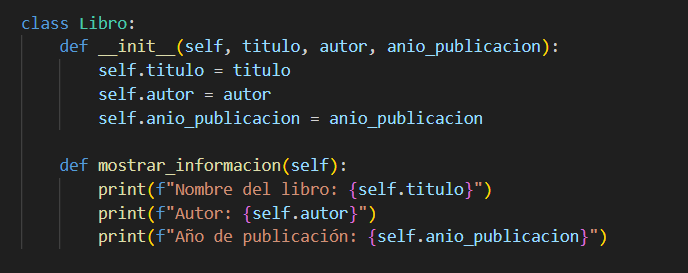
\includegraphics[width=0.7\linewidth]{images/12.png}
    \caption{Creando la clase Libro}
    \label{fig:enter-label}
\end{figure}

\begin{figure}[H]
    \centering
    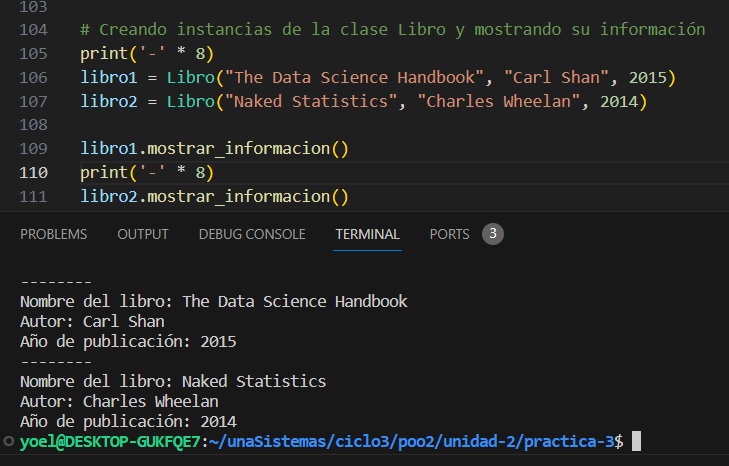
\includegraphics[width=0.7\linewidth]{images/12-1.png}
    \caption{Creando dos instancias de la clase Libro y mostrando su información mediante el método 'mostrar\_informacion()'}
    \label{fig:enter-label}
\end{figure}

\subsection{Modifica la clase Curso para que tenga una lista de estudiantes y métodos para agregar y eliminar estudiantes.}

\begin{figure}[H]
    \centering
    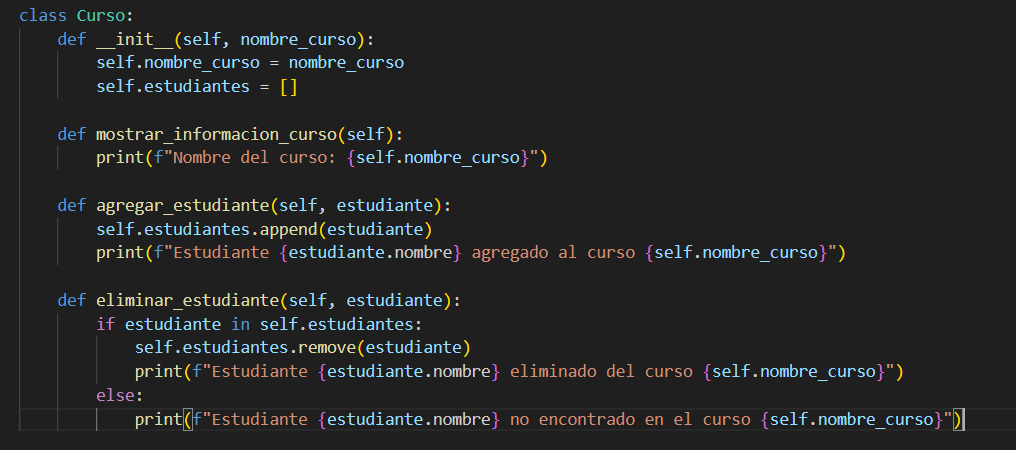
\includegraphics[width=1\linewidth]{images/13.png}
    \caption{Clase 'Curso' modificada para tener una lista de estudiantes y métodos para agregar y eliminar estudiantes}
    \label{fig:enter-label}
\end{figure}

\subsection{Crea una clase Profesor que tenga atributos como nombre y especialidad. Relaciona la clase Profesor con la clase Curso.}

\begin{figure}[H]
    \centering
    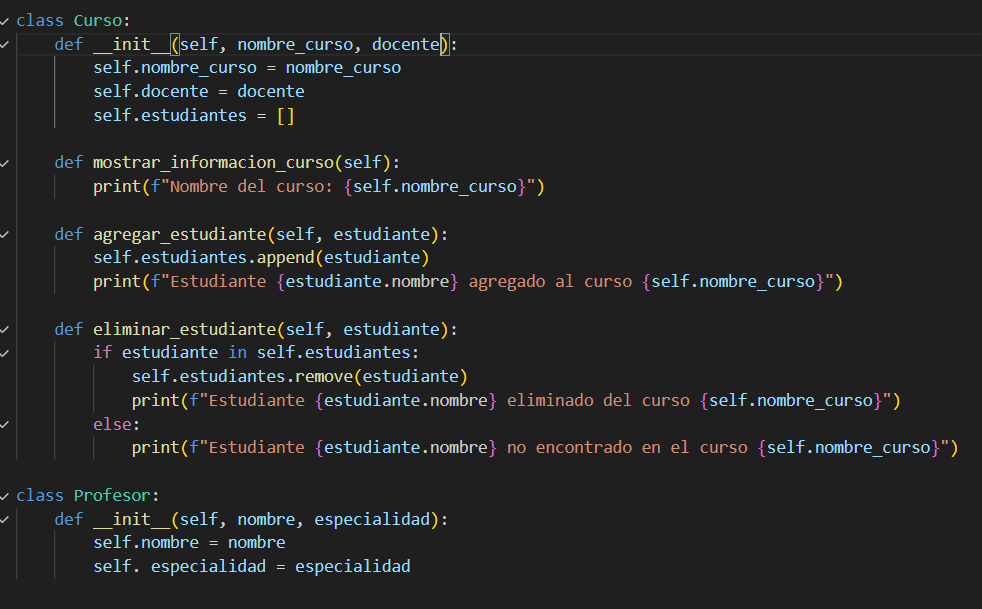
\includegraphics[width=1\linewidth]{images/14.png}
    \caption{Creando la clase Profesor con atributos de nombre y especialidad y modificando la clase Curso con un atributo adicional que representa al docente del curso}
    \label{fig:enter-label}
\end{figure}

\subsection{Implementa un programa que simule una situación en la que varios estudiantes se inscriben en diferentes cursos de una universidad ficticia.}

\begin{figure}[H]
    \centering
    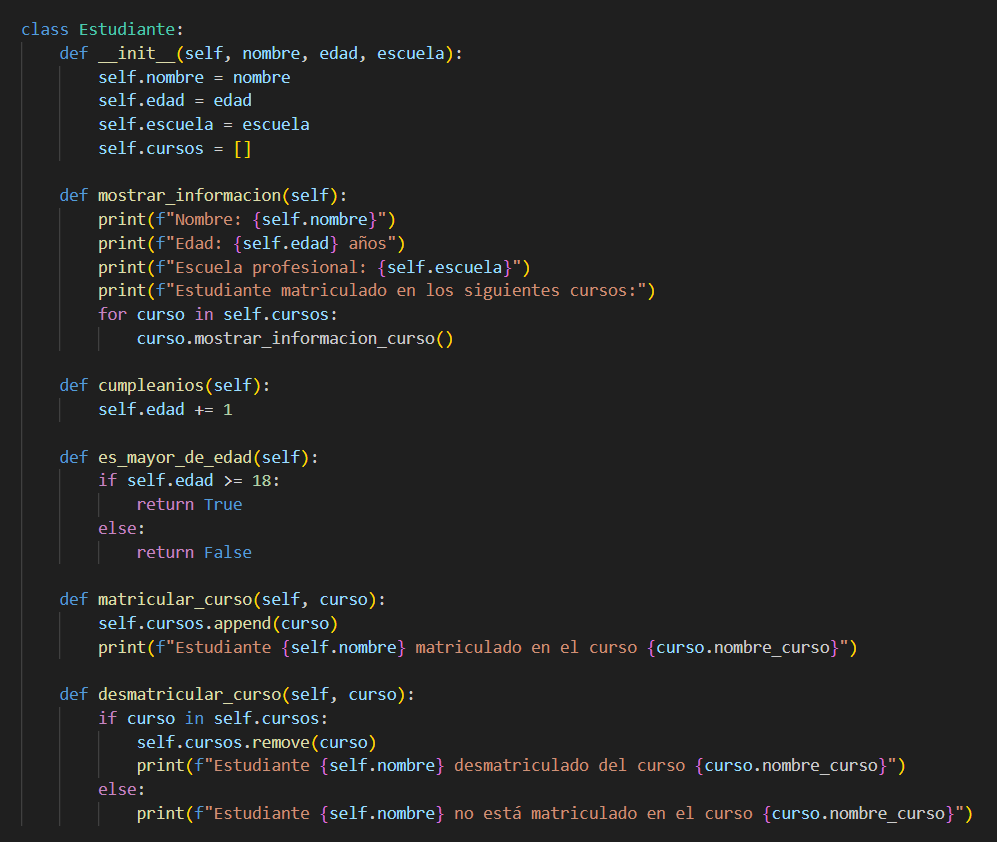
\includegraphics[width=1\linewidth]{images/15.png}
    \caption{Modificando la clase Estudiante para que tenga como atributo una lista de cursos en la que está matriculado y que tenga métodos para matricular y desmatricular de cursos}
    \label{fig:enter-label}
\end{figure}

\begin{figure}[H]
    \centering
    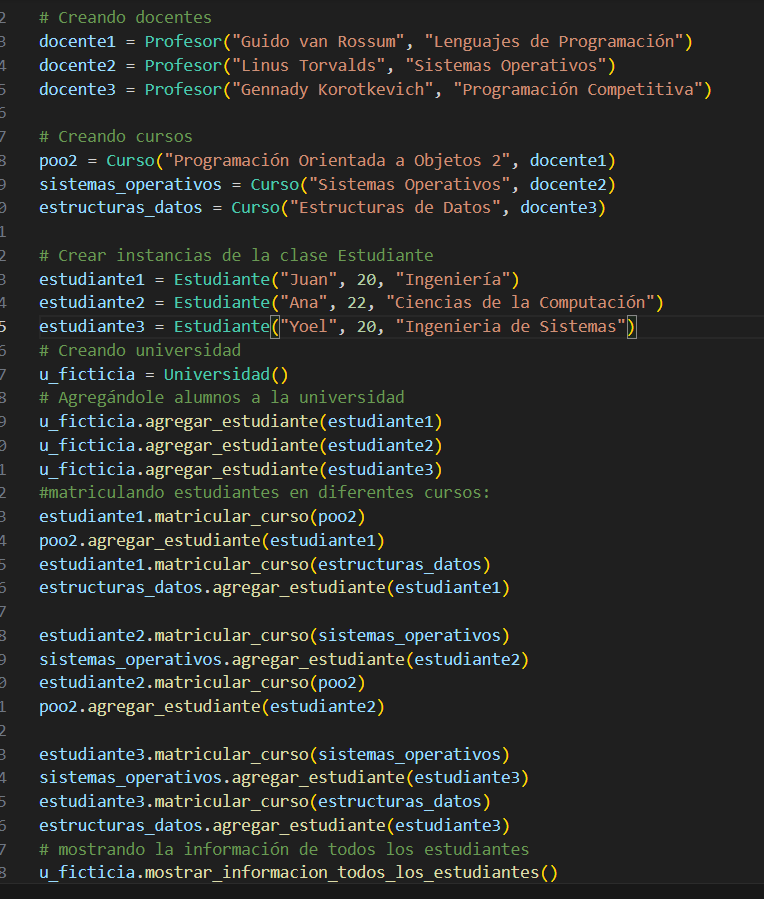
\includegraphics[width=1\linewidth]{images/16.png}
    \caption{Programa que simula estudiantes inscribiéndose en diferentes cursos}
    \label{fig:enter-label}
\end{figure}

\begin{figure}[H]
    \centering
    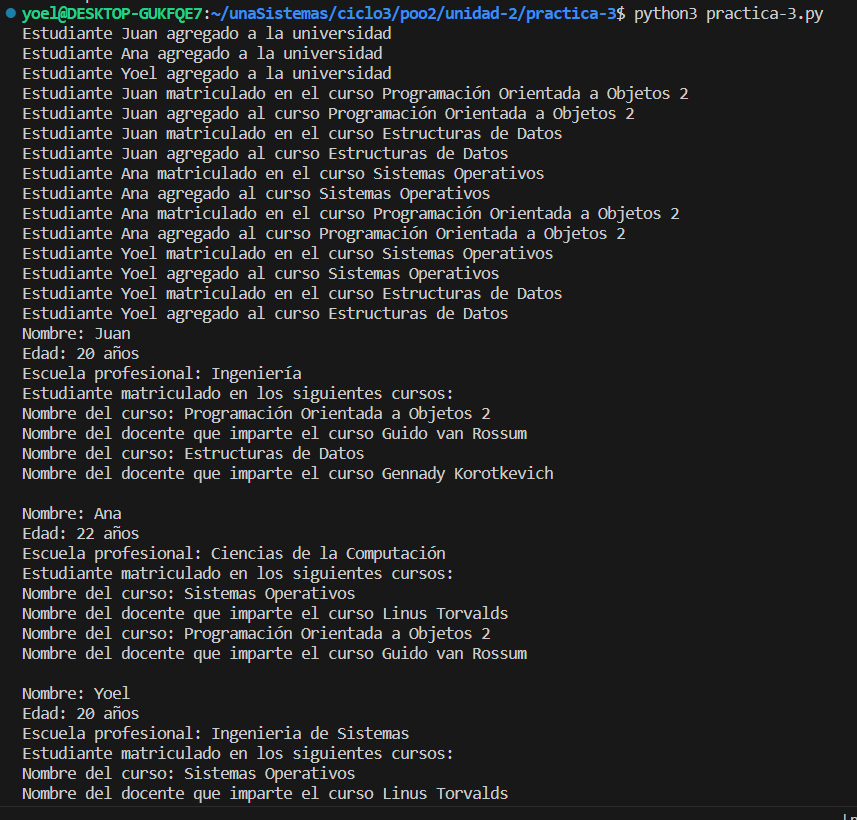
\includegraphics[width=1\linewidth]{images/17.png}
    \caption{Resultado en pantalla}
    \label{fig:enter-label}
\end{figure}

%para poner el código:
% \begin{sloppypar}
% \url{https://github.com/YoelCanaza/poo2-practica-2/blob/2289090a20512564e76f267bf34728590dbd6293/practica-2.py}
% \end{sloppypar}

\lstinputlisting[language=Python, style=mystyle, caption={Código con todas las modificaciones pedidas en los ejercicios}]{practica-3.py}


\end{document}